% ----------------------------------------
% State of the art
% ----------------------------------------

\chapter{State of the art}
\label{ch:state-of-the-art}

% TODO Begin elk hoofdstuk met een paragraaf inleiding die beschrijft hoe dit
% hoofdstuk past binnen het geheel van de bachelorproef. Geef in het bijzonder
% aan wat de link is met het vorige en volgende hoofdstuk.

% Pas na deze inleidende paragraaf komt de eerste sectiehoofding.

% Dit hoofdstuk bevat je literatuurstudie. De inhoud gaat verder op de inleiding,
% maar zal het onderwerp van de bachelorproef *diepgaand* uitspitten. De bedoeling
% is dat de lezer na lezing van dit hoofdstuk helemaal op de hoogte is van de
% huidige stand van zaken (state-of-the-art) in het onderzoeksdomein. Iemand die
% niet vertrouwd is met het onderwerp, weet nu voldoende om de rest van het
% verhaal te kunnen volgen, zonder dat die er nog andere informatie moet over
% opzoeken.

\section{Distributed development}

In a technology landscape that has long been shifting to meet the current trends
of economic globalization, software development has evolved from being mostly
concentrated at a single location, to being geographically distributed around
the globe. 

According to \textcite{Yuhong_2008}, the terms \gls{gdd}, \gls{gdd2} and
\gls{gsd} are mostly used to refer to the same distributed development model. In
the remainder of this thesis, the term \glsacronymnfirst{gdd} will be used mainly
when emphasis is required on the geographical aspect of the distributed
development model.

The application of \gls{gdd} can be done in many distinct ways. One way is in
the form of \textbf{\gls{outsourcing}} agreements, often with countries where
employment costs are more economically beneficial.

Another way, is the separation of a company into different local
\textbf{divisions} or departments in different cities. This envelops both large
multinational companies that operate around the globe, or more
nationally-focused companies that have different branches in different cities.
\autocite{Kiel_2003} This also includes the practice of \textbf{\gls{offshoring}},
which tends to have the same motivations as outsourcing, but keeps control in
the hands of the business, and does not involve a third party \autocite{Oshri_2015}.


\subsection{Benefits}

Companies often have a plethora of different business reasons to distribute the
development, maintenance and management of software. 

\begin{itemize}
    \item Financial benefit (labor costs, taxation, ...)
    \item Market insight: local teams have more insight into local trends
    \item Talent availability: a larger pool of skilled developers is available,
    potentially even with different specializations in different locations.
    \autocite{Conchuir_etal_2009}
    \item Faster time-to-market: because development can be distributed across
    multiple timezones, a \gls{fts} workflow could potentially increase
    development speed drastically\footnote{According to
    \textcite{Conchuir_etal_2009}, \gls{fts} workflow is however practically
    almost inachievable, and in practice, many companies even make sure the time
    zones overlap as much as possible, to reach better inter-team communication.
    } \autocite{Carmel_2010}.
\end{itemize}

\subsection{Challenges}

While the aforementioned benefits of \gls{gdd} appear very useful in theory, on
the practical side, there are of course some challenges to this approach. For
example, according to \textcite{Smite_etal_2010}, implementing an \textbf{agile
methodology} within a distributed software development model is not
straightforward; and the characteristics of agile and distributed development
could be seen as polar opposites. 

But the idiomatic \textit{``elephant in the room''} is \textbf{communication}.
In projects where teams are located together, communication can be rather
informal, which helps team members more rapidly gain project and technical
knowledge, as well as knowledge of the more human aspects of their coworkers,
such as working style and expertise. According to \textcite{Sengupta_2006},
frequency of communication has an inverse relationship to physical separation of
team-members, and in multi-site environments, the decrease in communication
frequency is so sharp, that informal communication is nearly nonexistent.
Pairing this with \textbf{cultural} and timezone differences, makes all
communication very difficult when practicing \gls{gdd}.


\subsection{The role of the architecture in enabling distributed development}

According to \textcite{Yuhong_2008}, in a \gls{gdd} environment, establishing
and maintaining a common software and/or solution architecture that can support
a distributed development model, is key for the success and sustainability of
the software project. Among other architectures, she describes a module-based
project architecture, where self-contained software components are developed
independently. This way, teams could develop these modules simultaneously,
without a large interdependence on other modules. This, however, requires strong
decoupling of the software modules.\newpage
\section{The evolution from \gls{monolithic} to distributed architectures}

The development of applications for the web has seen some dramatic shifts over
the years. Apart from new technologies, protocols, and standards, the way web
applications are structured has undergone some evolutions as well. ``Software
architecture'' not only outlines the pure structure of the application but also
defines the responsibility of all the pieces of the application, and how these
pieces ought to interact with each other \autocite{Fedorov_etal_1998}.


\subsection{\Gls{Monolithic} architecture}

Historically, one of the earliest architectures for implementing web
applications was the \textbf{client-server model}. The service provider or
\textit{server} can share its resources with service users called
\textit{clients}. According to \textcite{Reese_2000}, at the time, most web
applications were simple two-tier client-server applications. The web browser on
the client-side retrieves data and files from the data store at the webserver
side, without much data interpretation or manipulation. The upcoming increase of
the computing power of hardware, made it possible to execute some data
processing on the client-side, using for example technologies like Java. 

Although two-tier server-client architectures were quick to set up and had
robust tooling, a pretty significant downside got introduced: these so-called
\textit{fat clients} were now not only concerned with the task of presenting
data to the user, but are also bloated with business logic and data processing.
Conversely, any change in business rules would also require every client to adapt
to this change. \autocite{Gallaugher_Ramanathan_1996}.

A \textbf{three-tier} architecture was conceptualized in an attempt to overcome
the downsides of the two-tier approach. The idea sounds not very groundbreaking:
just introduce the handling of business logic on the server-side, rather than on
the client. This results in the following tiers \autocite{Aarsten_etal_1996}:

\begin{itemize}
    \item The client tier (also known as the presentation tier), which contains
    the \gls{gui}
    \item The application tier (also known as the business tier or logic tier),
    i.e. the application servers that contain objects representing business
    entities and domain logic.
    \item The data(base) tier that handles the storage of domain objects and data.
\end{itemize}



% two-tier vs three tier figure here? 

With the introduction of this physical seperation, the next challenge was the
structure of the sotware's code.  

Over an extensive period, applications built on top of the client-server model
extensively used the \textbf{\gls{mvc} pattern} \autocite{Pavlenko_etal_2020}. Like the
name suggests, this pattern describes 3 parts, that are used as conceptual and
architectural separations in the software. The business logic of the application
is encapsulated in the \textbf{model}, the presentation logic is the
responsibility of the \textbf{view}, and the \textbf{controllers} handles the
the user actions in the view, and connects these actions to the appropriate
models and updated views.

However, according to \textcite{Leff_Raylfield_2001}, implementation of the
\gls{mvc} pattern for web applications in a client-server environment, brings up
the question of partitioning between servers and clients. Instinctively it is
clear that the views belong to the client and the models belong to the server,
but for the controllers, this separation is not so clear. Assigning the
controllers to the client-side would result in a \textit{fat client} again,
while assigning them to the server-side (the \textit{thin client} approach)
would often mean too many round-trips to the server must be performed on every
request. In practice, the workaround for this partitioning is a \textit{dual
\gls{mvc}} approach, which partitions the controllers between the client and the
server.


While the \gls{mvc} architecture pattern can give developers a cleaner
seperation of concerns in their code, it still produces a \textbf{tightly
coupled} solution. Any change would still mean the entire code would have to be
rebuilt and redeployed \autocite{Fowler_Microservices_2014}. This significantly
reduces development speed, as well as agility. \Glsplural{monolith} can also be considered
a  ``single point of failure'': whenever one part of the software is
malfunctioning, the whole system is crippled.


\subsection{The split stack development model}


In more recent times, developer teams started to adopt \textbf{split stack
development}, where the \gls{gui} is handled in the so-called ``\gls{frontend}'' and
the business and data logic are dealt with by a ``\gls{backend}'' system. The
communication between these two parts can be carried out in multiple ways, but
one of the most common ways is via a (RESTful) \gls{api}.

%TODO figure

Decoupling the frontend presentation logic from the \gls{backend} business logic
introduces some major benefits: \autocite{Dunkley_2016}
\begin{itemize}
    \item \textbf{Multiple clients}\\
    As it is not at all concerned with presentation logic, the same
    \gls{backend} service can now serve data to multiple different clients (e.g.
    web, desktop, mobile,...). To support a new type of client, only
    presentation logic has to be implemented. 
    %
    \item \textbf{Specialized teams}\\
    The split of \gls{frontend} and \gls{backend} allows developers to
    specialize themselves in these fields, yielding a deeper knowledge of the
    selected fields. 
    %
    \item \textbf{Independent technology stacks}\\
    Tying in with the previous point: as teams specialize, they desire and/or
    require more specialized technologies. The decoupling of front- and
    \gls{backend} removes any restraints on technology selection between the two
    areas. For example, \gls{frontend} developers can use client-side
    technologies and frameworks such as Typescript and React, while
    \gls{backend} developers can leverage server-side technologies such as .NET
    or Java. This also makes each individual solution more future-proof. 
    %
    \item \textbf{Simultaneous development}\\
    As a result of all outlined benefits above, and the basic concept of
    decoupling, teams can work independently, autonomously and therefore
    simultaneously. For example, a change to the visual styling of a website,
    will not require any of the server-side code to change, and will also not
    trigger a rebuild there.
    %
    \item \textbf{Independent deployment and scaling}\\
    While a \gls{monolith} had to be deployed as one big program, teams could now
    deploy the \gls{frontend} and \gls{backend} solutions according to their
    needs. Often a static hosting solution is enough to publish a client, while
    a \gls{backend} service might need some serious infrastructure to remain
    operational.
\end{itemize}

% TODO callback to distributed development?

Of course, these benefits also come at the cost of some drawbacks. 

Firstly, the contract between the \gls{frontend} and \gls{backend} teams is a
well documented \gls{api} with clearly defined \glsplural{endpoint}. For RESTful
web \gls{api} \textbf{documentation}, the OpenAPI
specification\hreffootnote{https://www.openapis.org/}, which is also known as
\textit{Swagger} documentation, provides a standardized way of defining this
contract \autocite{Koren_Klamma_2018}. Of course, time and effort needs to be
spent creating robust documentation. 

Secondly, breaking changes have to be avoided at all times. \Gls{frontend} code
might depend on backend \glsplural{endpoint} that will get deleted in an
upcoming update. This is not acceptable.
\textbf{Versioning}\hreffootnote{https://restfulapi.net/versioning/} provides a
way to keep supporting clients that rely on a version of the \gls{api} before
the breaking change was made.

Lastly, more relevant in the context of this thesis: while dividing the
\gls{frontend} from the \gls{backend} does provide benefits; in large, rapidly
scaling applications, it simply isn't enough. After a
\gls{frontend}-\gls{backend} split, one does still end up with a both a
\textbf{\gls{monolithic} \gls{backend}} and a \textbf{\gls{monolithic}
\gls{frontend}}. 

Shifting the frame of reference to the server-side: the \gls{backend}
\gls{monolith} still posesses the same downsides the overall \gls{monolith} had
introduced: one change in the logic and the entire application has to be
rebuilt and redeployed. Also, the issue of scaling still persists: the server
can be updated with more powerful hardware (vertical scaling) or the \textit{entire}
server-sice application can be replicated on different servers, with a
\gls{load-balancer} deciding how to distribute incoming requests (horizontal scaling).
Keyword here is \textit{``entire''}, as no specific part of the server-side
application can be scaled up indendently. 

\newpage
\section{Microfrontends}

With the introduction of the \gls{ma} pattern, \gls{backend} systems can be
split up into multiple services, each with their own responsibilities. As
previously described, this can bring great benefit. However, even after a
transition to \glsplural{microservice} on the server-side, the client-side
applications using these services are mostly still \gls{monolithic} in nature.

A \gls{monolithic} \gls{frontend} does not have to be a problem.
\Glsplural{monolith} are quick and easy to set up, and historically, most of the
heavy lifting was done on the server-side anyway. However, the complexity of
client-side applications has seen a drastic increase over the last few years.
This can be attributed to many factors: increased hardware and web browser
capabilities, a wide variety of client devices, massive market growth for
digital services, and the web transitioning from a document platform to the
largest application platform \autocite{Ball_2019}; just to name a few.

In these complex applications, the downsides of a \gls{monolithic} architecture
come back into view: every change requires the entire \gls{frontend} application
to be rebuilt and redeployed, codebases grow very large in size, etc... Even
worse, because the client-side application has a functional dependency on the
server-side application, a small change in one particular area of the
\gls{backend} logic could also trigger a change in the \gls{frontend}, causing
the entire \gls{frontend} to yet again be rebuilt and redeployed
\autocite{Rappl_LogRocket_2019}.

There is also the issue of \textbf{domain knowledge}: while the \gls{ma} gives
\gls{backend} teams the possibility of focussing on one specific part of a
business domain, teams that are developing the client-side code are still
expected to know the entire scope of the application. Often this means a
reliance on personal inter-team communication, which in larger organizations
tends to be expensive \autocite{Geers_2020}. 

While component-based paradigms introduced by libraries and frameworks (such as
React\hreffootnote{https://reactjs.org},
Angular\hreffootnote{https://angular.io} and
Vue\hreffootnote{https://vuejs.org}) can alleviate some of the complexity of the
current \gls{frontend} systems, they still do not enable  fully autonomous, decoupled,
modular and/or distributed development of large web applications.

\subsection{What are microfrontends?}

In 2016 the ThoughtWorks Technology Radar \autocite{ThoughtWorks_2020} coined
the term ``\textit{Micro Frontends}'' to describe the split of the
\gls{frontend} \gls{monolith} into independently deployable and maintainable
pieces. This new architecture pattern could therefore be regarded as an
extension of the \gls{ma} into the \gls{frontend} space.

The characteristics of the \gls{mfa} pattern are therefore very closely related
to those of the \gls{ma} pattern, as described in section
\fullref{principles-of-the-mfa}. Every individual \gls{frontend} module has a
relatively small codebase, is focussed around one specific domain or company
mission, and should be modular, decoupled and independently developed; most
optimally by autonomous teams.

A visual representation of the \gls{mfa} pattern is shown in
Figure~\ref{fig:microfrontends}.


\begin{figure}
  \centering
  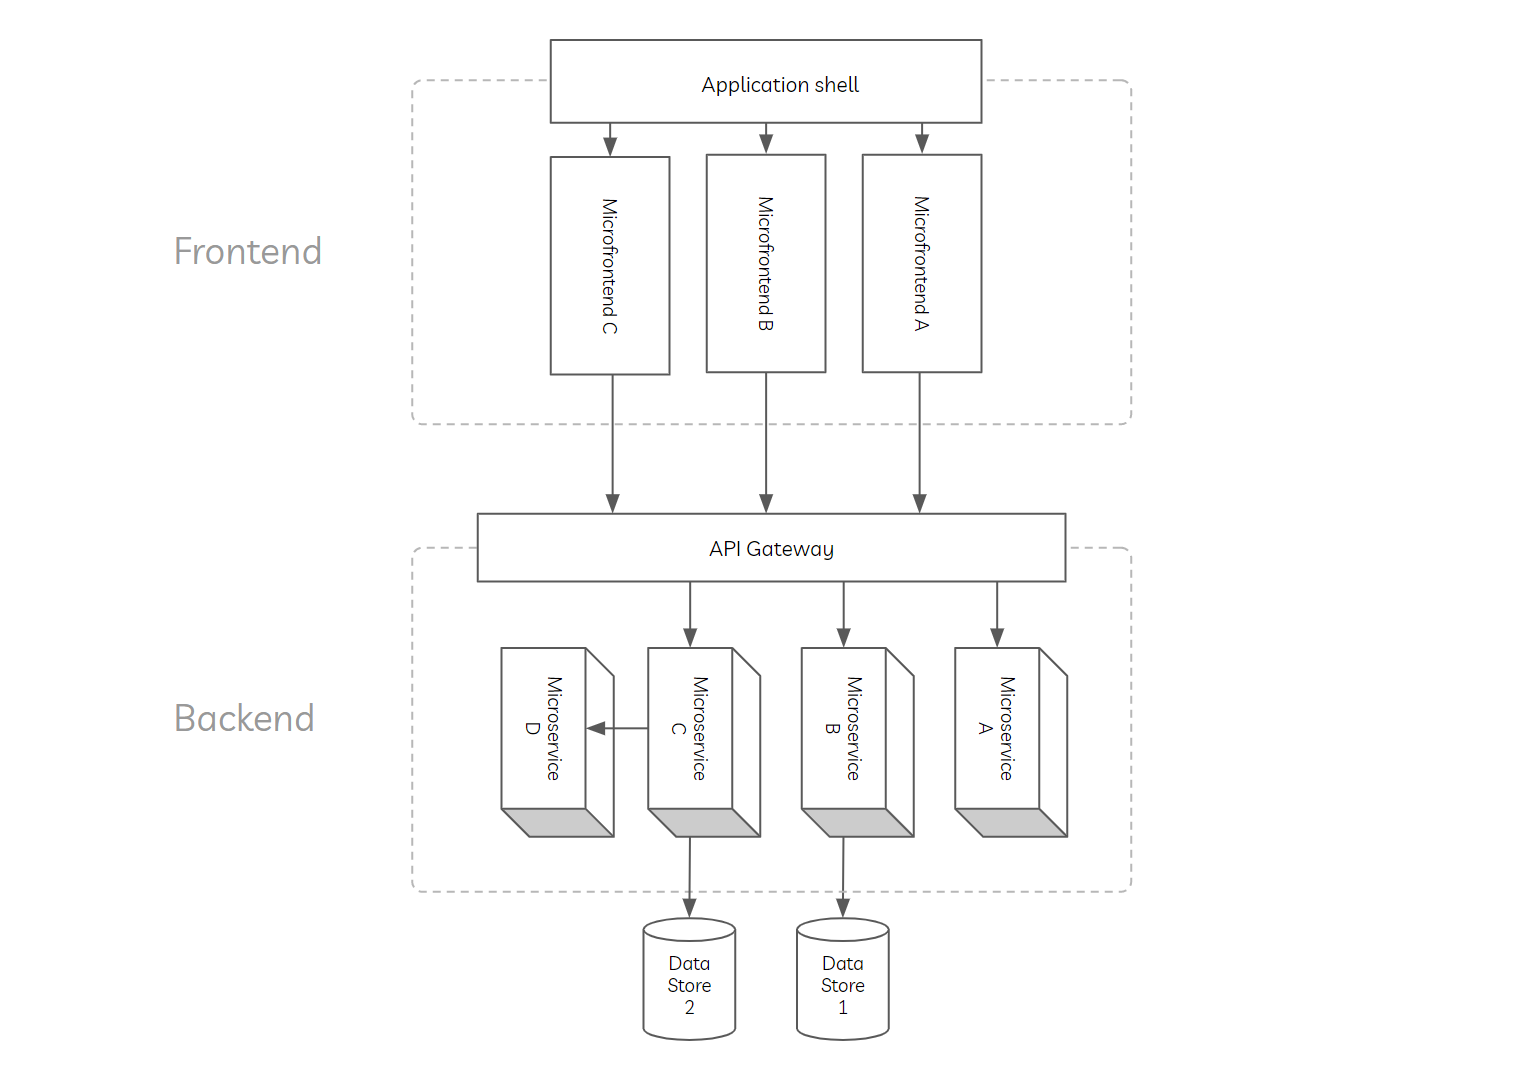
\includegraphics[width=\textwidth]{microfrontends.png}
  \caption[Microfrontends]{A diagram showing an example of a
  \gls{mfa}.}
  \label{fig:microfrontends}
\end{figure}

\subsection{How do microfrontends enable distributed development?}

A significant difference between \glsplural{microfrontend} and other software
architectures is the impact on \textbf{team structure} and organizational shift
\autocite{Geers_2020}. So, while \glsplural{microfrontend} have lots of
technical aspects to consider, it is important to reflect on the organizational
aspects first.

As discussed in \fullref{ssec:microservices}, when adopting the \gls{ma}, a shift
has to be made to smaller independent teams around a specific business need.
However, this only brings about changes in the \gls{backend} teams, while the
\gls{frontend}-oriented development team will usually not follow suit. This
keeps the overarching team structure ``horizontal'': divided per layer or
technology.

One of the benefits of horizontal teams is that this structure enables experts
focussing on specific technologies to co-operate together as one team. This way,
they can ensure a high technical standard within the boundaries of their
respective areas of expertise.

In geographically distributed teams, the consequence could be that these
technical teams operate from entirely different locations. According to
\textcite{Smite_etal_2010}, this can result in compatibility issues between software
layers and a less customer-focused development model. Moreover, disputes can
arise between the different teams because no team has full responsibility for
the delivery of any feature.

\subsubsection{Feature teams}
\label{feature-teams}

To mitigate the issues arising from geographically distributed horizontal teams;
multidisciplinary or cross-functional ``feature teams'' can be introduced. These
are grouped around a specific business case or customer need. This ``vertical
slicing''  enables teams to be more independent and have end-to-end
responsibility for the features they develop.

This feature team approach has multiple advantages: \autocite{Smite_etal_2010}
\begin{itemize} 
  \item \textbf{Optimized feature development}\\
  Focussing on features instead of technical details aids in delivering the
  highest amount of business value.
  % 
  \spacedItem \textbf{Decreased need for ``expensive'' communication}\\
  Communication within a team is usually faster and more informal than
  communications between teams, especially if teams are geographically
  distributed. Since a feature can be developed by a single team, the need for
  expensive communication decreases.
  %
  \spacedItem \textbf{Greater sense of developer involvement}\\
  According to \autocite{LarmanVodde_2008}, developers who operate in a feature
  team feel a greater sense of ownership and accountability for the features
  they develop. 
  %
\end{itemize}

It is worth mentioning that these benefits combined can result in a faster cycle
time and thus an increase in development speed \autocite{Geers_2020}.

On the other side, this approach also comes with caveats. One of them is the
danger of compromising on the \textbf{conceptual integrity} of the software
systems. More time will have to be spent up-front laying a solid foundation for
conventions and standards. The effort to then maintain the consistency of the
software system is usually where the software architect has a key role. In
larger projects, a technical service team can be assembled to provide technical
coherence across different distributed systems \autocite{Smite_etal_2010}. While
this is something to consider, this also means an increased emphasis on better
code quality right from the start, which could prove very beneficial in the long
term \autocite{LarmanVodde_2008}.

Another caveat is that, especially in large corporations, \textbf{changing the
complicated organizational structure} might not be possible, or at the very
least slow and difficult.

\subsection{Common implementation patterns}
\label{ssec:mf-implementation-patterns}

As is the case with lots of architectural patterns, there are many ways of
implementation possible. With the \gls{mfa}, this is also the case. Various
options differ in complexity, goal, and mechanism. 

\Glsplural{microfrontend} often need to be composed to be able to reach a
coherent application. Every \Gls{microfrontend} brings its own \textbf{pages}.
Often, \glsplural{microfrontend} also expose reusable components to be rendered
in a variety of locations, to provide functionality. These are often called
\textbf{fragments}.

Below some of the possible implementation and composition techniques are
outlined.

\subsubsection{The \textit{web approach}}

The most straightforward way of leveraging the \gls{mfa} pattern is by not using
any integration technique at all. Instead, there can be opted for mechanisms
that exist in the world of the web. 

As described by \textcite{Rappl_2021}, the \textit{web approach}'s main
mechanism for \gls{microfrontend} reference is by way of their \gls{url}.
\textbf{Hyperlinks} can be used to let the user navigate between different
\glsplural{microfrontend}. This, however, compromises on user experience and
usability. With this approach, for example, elements from multiple
\glsplural{microfrontend} cannot be rendered on the same page. 

To enable visual composition of \glsplural{microfrontend} in the most
straightforward way, \textbf{\glsplural{iframe}} can be used. By using an
\texttt{<iframe>} tag with a \texttt{src} attribute that points to a \gls{url},
one could embed visual components of one \gls{microfrontend} (fragments) within
another, without sacrificing on strong isolation between the two
\autocite{Geers_2020}. The disadvantage here is the notoriously bad
characteristics of \glsplural{iframe}. One of these is bad performance:
according to \textcite{Souders_2013}, \glsplural{iframe} are up to 2 orders of
magnitude more expensive to create than any other \gls{dom} element. Moreover,
iframes also block the loading process of the rest of the page. Other suboptimal
characteristics include accessibility and \gls{seo}.

The simplicity of the web approach is also where it lacks applicability for
larger projects. One of the biggest reasons to implement
\glsplural{microservice} and \glsplural{microfrontend} is scalability, which the
web approach is often not very suitable for.

\subsubsection{Server-side composition}

To accommodate for scalability and ensure higher performance, the composition of
the \glsplural{microfrontend} can be done before even reaching the end user's
web browser. This will require dynamically composing the application on the
server-side.

According to \textcite{Geers_2020}, this server-side composition can also
provide a solid basis to be able to enable \gls{pe}, and is a big advantage for
\gls{seo}.

There are multiple techniques to enable server-side composition. These include,
but are not limited to:
\begin{itemize}
  \item \textbf{\gls{ssi}}.\\
  This uses an \textit{\gls{ssi} directive} (a HTML comment) to signify a
  placeholder for fragments to be rendered into.
  \begin{minted}{html}
<!-- #include virtual="/fragment" -->
  \end{minted}
  It also supports the execution of commands from the server, and even some
  conditional logic \autocite{Apache_2013}. \gls{ssi} has been around for a long
  time, this way most web servers have support for it. Because its directives
  are HTML comments, using these on a server that is not configured for
  \gls{ssi} won't crash the application (the fragment will just simply not be
  rendered).
  %
  \spacedItem  \textbf{\gls{esi}}.\\
  Instead of HTML comments, \gls{esi} uses \gls{xml}-based \gls{esi} tags:
  \begin{minted}{xml}
<esi:include  src="/fragment" 
              alt="/fallback" 
              onerror="continue" />
  \end{minted}
  \gls{esi} has a more extensive amount of functionalities (error handling,
  fallbacks, ...) compared to \gls{ssi}. It is however more difficult to
  implement, because while \gls{ssi} can work for nearly all web servers,
  \gls{esi} requires more specialized set-ups that are more complex to configure
  \autocite{Rappl_2021}.
\end{itemize}


\subsubsection{Client-side composition}

While with server-side composition, a web server was used as an aggregation
layer for integrating the \glsplural{microfrontend}; with client-side
composition, the goal is to put this responsibility onto the end user's browser
itself. The browser will have to render one parent HTML document which contains
the instructions to integrate all the individual \glsplural{microfrontend} into
itself.

This parent HTML document is often called the \textbf{\gls{appshell}}
\autocite{Geers_2020}\autocite{Rappl_2021}. 

The \gls{microfrontend} scripts and resources are often served from a
\textbf{\gls{cdn}}.

Client-side composition can be done in various different ways. A selection is
outlined below:
\begin{itemize}
  \item \textbf{Web Components}\\
  According to \textcite{Mozilla_WebComponents}, this term encompasses three
  main technologies, namely custom elements, shadow \gls{dom} (that can provide
  reusable \gls{dom} trees to ensure isolation) and HTML templates.
  % 
  \spacedItem \textbf{\gls{spa} composition}\\
  In recent years, client-side frameworks have become the staple of fast and
  app-like experiences on the web. Most of these frameworks introduce a custom
  client-side routing solution. When using \gls{spa} composition, the
  \gls{appshell} needs to take responsibility for the routing. The
  \gls{appshell} will now not just render fragments using HTML, but execute
  scripts defined in the \glsplural{microfrontend} themselves to be able to
  integrate them.
\end{itemize}

Client-side composition is great for delivering highly interactive, dynamic web
applications. However, because the application is not served to the browser in
full, the downsides include suboptimal \gls{seo} and an increased time to first
load.

\subsubsection{Universal composition}
\label{sssec:universal-composition}

Aiming to combine the client-side and server-side composition approaches, and
get the advantage of both, a hybrid approach can be achieved. Universal -- or
\textit{isomorphic} -- composition describes the process of 
\begin{enumerate}
  \item composing the application on the server-side, providing a fast initial
  load and thus enabling \gls{pe} and optimal \gls{seo}
  \item \textit{hydrating} the application so it becomes fully client-side
  interactive, providing the benefits of a highly dynamic application.
\end{enumerate}


\subsection{Usage of microfrontends}

\Glsplural{microfrontend} are being used by companies all over the world.
Swedish furniture company IKEA mainly uses autonomous vertical teams that can
develop in different technologies if necessary \autocite{Stenberg_2018}.
Spotify, a music streaming service provider from that same country, uses
\gls{iframe}-based \glsplural{microfrontend} within its desktop application to
be able to develop different parts from the same view independently. These
so-called \textit{Spotlets} are developed by \textit{Squads}, independent
cross-functional teams \autocite{Gall_2018}. German e-commerce fashion retailer
Zalando even created ``Project Mosaic''\hreffootnote{https://www.mosaic9.org/},
which contains a plethora of libraries and services to create both
\gls{frontend} and \gls{backend} \glsplural{microservice}.



\subsection{Benefits of microfrontends}

The \gls{mfa} carries over a lot of the advantages of the \gls{ma}
\autocite{Jackson_2019}: \textbf{technology independence} is now also possible
across different \gls{frontend} teams, allowing them to select the best tools
and frameworks for the job. Loose coupling enables the \textbf{scalibility} of
both the \gls{frontend} and \gls{backend}. Now, the \gls{frontend} can also
enjoy the benefits of independent deploys, isolated risks, and smaller
codebases.

\textbf{Teams} also benefit greatly and can be reorganized to even greater
benefit, as was discussed in detail in section \fullref{feature-teams}.

These factors can have great results for a business. Due to their loose
coupling, isolated features, and independent deployments,
\glsplural{microfrontend} can have vastly different release cycles, and
iteration and \textbf{feature development} is usually faster because the teams
don't have to wait for each other \autocite{Geers_2020}. \textcite{Rappl_2021},
because there is an existing composition mechanism, different
\glsplural{microfrontend} can be served to different users, enabling the
introduction of \textbf{A/B testing} without significant changes in the
\glsplural{microfrontend} themselves.

\subsection{Downsides and challenges of microfrontends}

However, to use the words of Cam \textcite{Jackson_2019}: \textit{``there are no
free lunches when it comes to software architecture - everything comes with a
cost''}. The \gls{mfa} does indeed come with a significant amount of tradeoffs
that need to be considered. 

\textbf{Organizational complexity} might be one of the biggest downsides of the
\gls{microfrontend} approach. This makes \glsplural{microfrontend} harder to
recommend to small development teams and companies. \textbf{Domain decoposition}
is often difficult and relies on a lot of organizational and technical factors. 

\textbf{Operational complexity} also increases: debugging, logging,
monitoring... all get a lot more complicated. Communication between the
different \glsplural{microfrontend} is generally also way more complex. If the
\gls{microfrontend} solution introduces the need for an \gls{appshell}, this
needs to be closely managed since it introduces a new single point of failure.

Lastly, lots of challenges are inherited from the \gls{ma}, as described in
\textit{``\nameref{sssec:microservice-challenges}''}.

\newpage
\section{Blazor WebAssembly}

On the 6th of February 2018, Daniel Roth -- Program Manager on the ASP.NET team
at Microsoft -- released a blog post called \textit{A new experiment:
Browser-based web apps with .NET and Blazor}. In this post, \textcite{Roth_2018}
announces an experimental project from the ASP.NET team: a component-ori\"ented
web \gls{ui} framework based on C\#, .NET, HTML and so-called Razor pages. 

The promise that was outlined by this post was a way to enable developers to
write web applications using .NET technologies, rather than resorting to
Javascript\footnote{Javascript is an implementation of the ECMAScript
specification. Read more on \hrefself{https://ecma-international.org/tc39}}, the
primary scripting language used on the web.

Executing .NET binaries within a web browser is made possible by
\textbf{\gls{wasm}}\hreffootnote{https://webassembly.org/}, a binary instruction format.
\Gls{wasm} has been added to the \gls{w3c} recommendation list, and has become
the fourth language to run natively in web browsers, alongside HTML, CSS and
Javascript \autocite{Couriol_2019}. 

An overview of how Blazor works is provided in Figure~\ref{fig:blazor-wasm}.

Rather than \gls{transpiling} every .NET assembly to \gls{wasm}, or relying on
plugins, Blazor just relies on a .NET runtime that can run inside the browser
sandbox, just like regular Javascript does. The current implementation of Blazor
uses the \gls{wasm}-compiled version of the
Mono\hreffootnote{https://mono-project.com/} platform -- an open source .NET
runtime -- as an \gls{il} interpreter to execute managed code at runtime.

Because of this, applications can leverage all standard web technologies like
websockets, the \gls{dom}, and all other browser \glsplural{api}, via
\textbf{\gls{jsinterop}}. It also ensures the various security protections put
in place by the sandbox environment to prevent malicious client-side attacks.

\begin{figure}
  \centering
  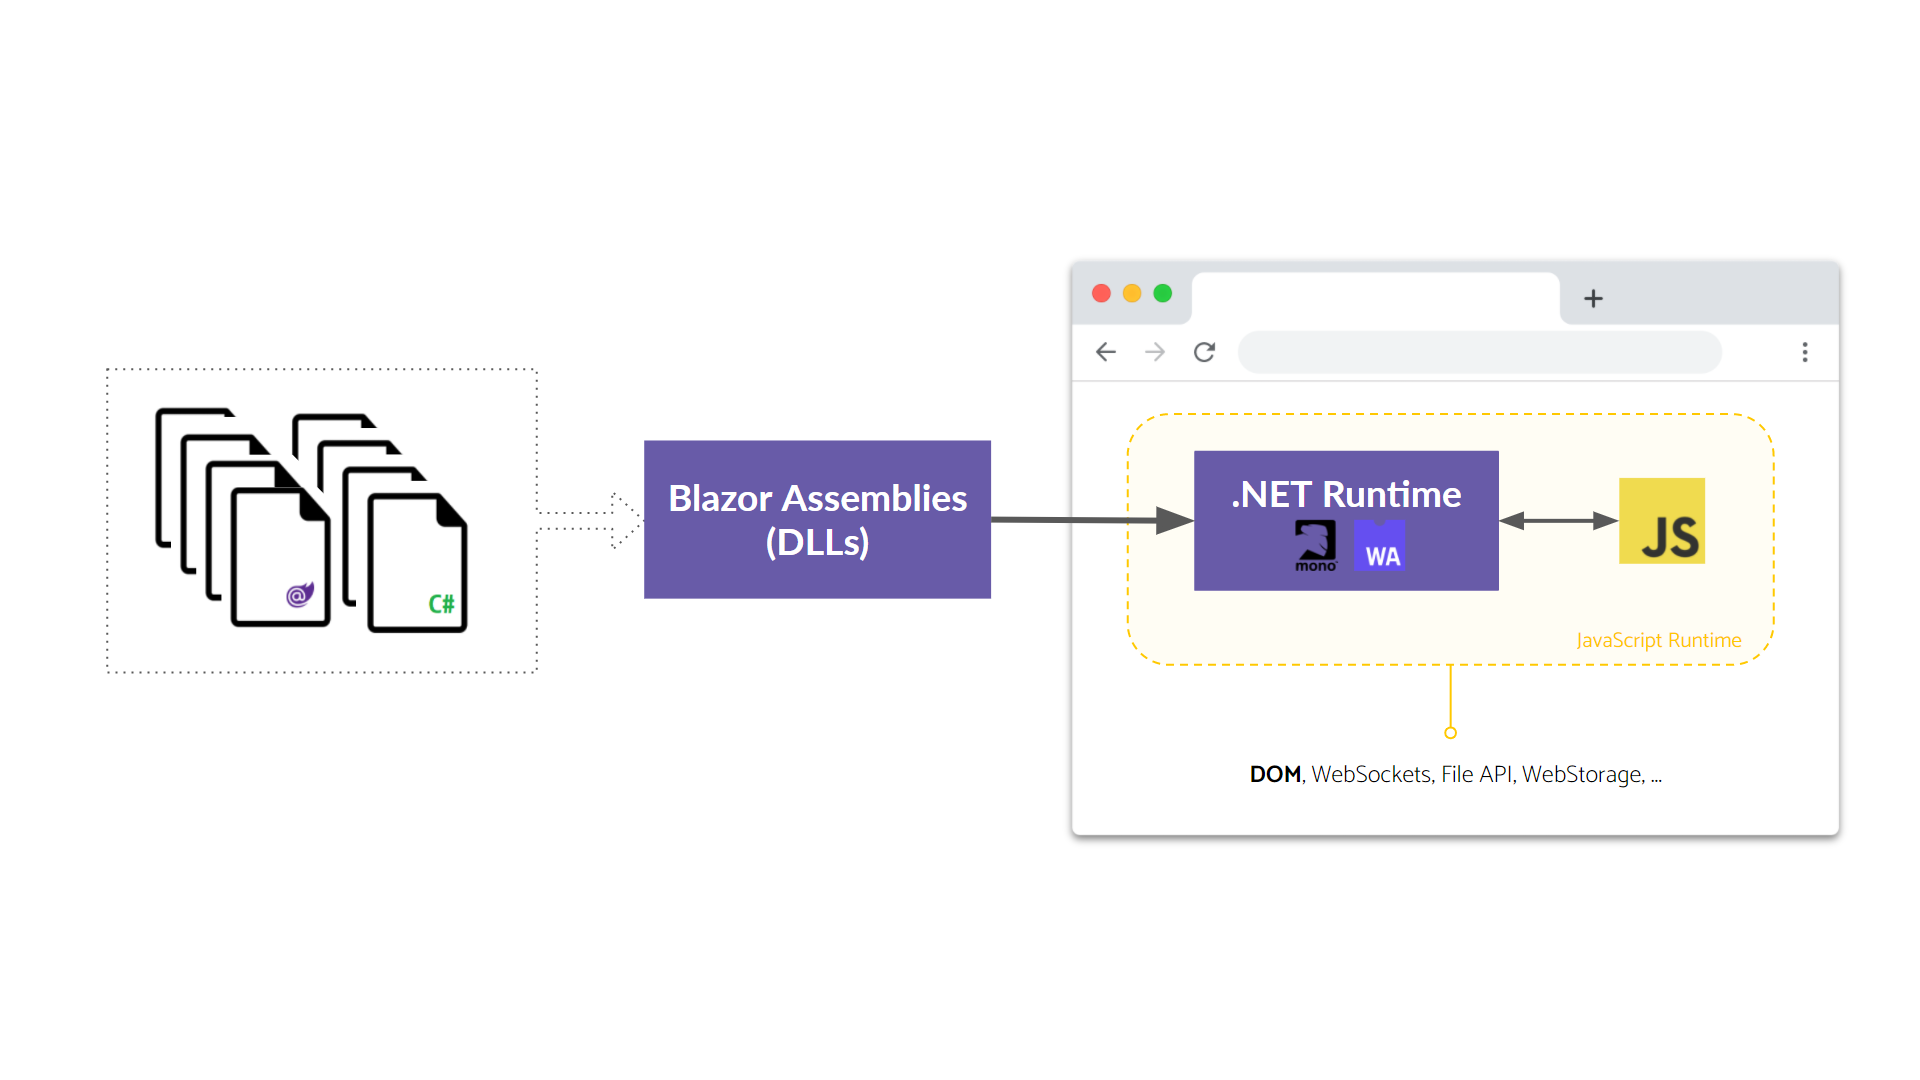
\includegraphics[width=0.8\textwidth]{blazor-wasm}
  \caption[Blazor WebAssembly]{A diagram that outlines how Blazor \gls{wasm}
  works. The C\# code and Razor files get compiled into \gls{il} assemblies, and
  run on a \gls{wasm} version of the Mono platform -- a .NET runtime -- inside
  the browser sandbox.}
  \label{fig:blazor-wasm}
\end{figure}


\subsection{Current state of Blazor and microfrontends}

According to \textcite{Rappl_MunichNETMeetup_2020}, an easy and effective way to
make distributed development possible in a Blazor \gls{wasm} project, is simply
to use separately distributed \textbf{component libraries}. In Blazor -- and in
the .NET ecosystem in general -- NuGet\hreffootnote{https://www.nuget.org} is
the standardized way of library distribution. One could create an \gls{appshell}
which imports and incorporates these NuGet packages. While this implementation
pattern makes development relatively straightforward, it has its downsides.

Because the integration happens at build-time; any change requires full
recompilation of the entire application. Also, upon startup, the \gls{appshell}
has to have full knowledge of all libraries, and they all have to be loaded for
the application to work, which makes this approach sub-optimal regarding
scalability. This integration method re-introduces coupling, and is generally
discouraged \autocite{Jackson_2019}.

Integrating \textbf{Blazor components in a JavaScript-based app shell} is
another option. While this has been done succesfully\footnote{See an example
here: \hrefself{https://github.com/lauchacarro/MicroFrontend-Blazor-React}}, and
there are already some frameworks that support this idea\footnote{For example
the Piral microfrontend framework with their \texttt{piral-blazor} converter.
See \url{https://piral.io}}, it is not within the scope of this thesis, as the
focus is on an almost exclusive .NET-approach.

\subsubsection{Challenges and potential solutions}

When looking for an approach that can dynamically load assemblies at runtime,
the client-side \textbf{routing} starts to present a problem. When defining a
page component in Blazor, the \texttt{@page} directive can be used. This will
later provide the generated class with a \texttt{RouteAttribute} with a value
that indicates the component's desired route template. The standard Blazor
router will then use reflection on the specified \texttt{AppAssembly} to scan the
loaded assemblies for these \texttt{RouteAttribute}s \autocite{Sainty_2019}.
This starts to become an issue if the assemblies are dynamically loaded -- and
thus not present upon compilation. 

Another challenge that can present itself is \textbf{debugging}. When running
Blazor DLLs on a \gls{wasm} runtime, a mechanism is needed to provide the link
between the browser and the debugging tools: the debugging proxy. According to
\textcite{Abdalla_2020}, this is a separate process that gets launched to load
so-called \gls{pdb} files. These are also called \textit{symbol} files, and they
are the link between the debugger and the source code \autocite{Microsoft_2021}.
Loading the \gls{microfrontend} symbol files dynamically is a challenge that
would need to be overcome to allow the debugging of Blazor applications using
\glsplural{microfrontend}.

These are challenges that would not come up when the composition would be done
at build-time like with component libraries. Luckily, the .NET 5 version of
Blazor introduces lazy-loading capabilities out of the
box\hreffootnote{https://docs.microsoft.com/en-us/aspnet/core/blazor/webassembly-lazy-
load-assemblies}, so most of these challenges that come from the dynamic loading
requirement can most likely be overcome. According to \textcite{Kdouh_2020}, the
Blazor router component, for example, now supports passing it additional
assemblies to consider. For debugging, the \texttt{AssemblyLoadContext} can
support the dynamic loading of dependencies with their symbols
\autocite{Microsoft_2019}. 
